\documentclass[10pt,a4paper]{article}
\usepackage[utf8]{inputenc}
\usepackage[english]{babel}
\usepackage{amsmath}
\usepackage{amsfonts}
\usepackage{amssymb}
\usepackage{graphicx}
\usepackage{natbib}
\usepackage{comment}
\usepackage[left=4cm,right=4cm,top=4cm,bottom=4cm]{geometry}
\title{Learning Structure in Time with a Plastic Recurrent Neural Network}
\makeatletter
\g@addto@macro\@floatboxreset{\centering}
\makeatother

\begin{document}
\maketitle
\section{Introduction}

We implemented a neural network consisting of binary neurons, modeled in discrete time steps, which follows the ideas presented in \cite{Duarte_2014}. The architecture of our network is depicted in Fig. \ref{fig:architecture} and shall be described in further detail.

\begin{figure}
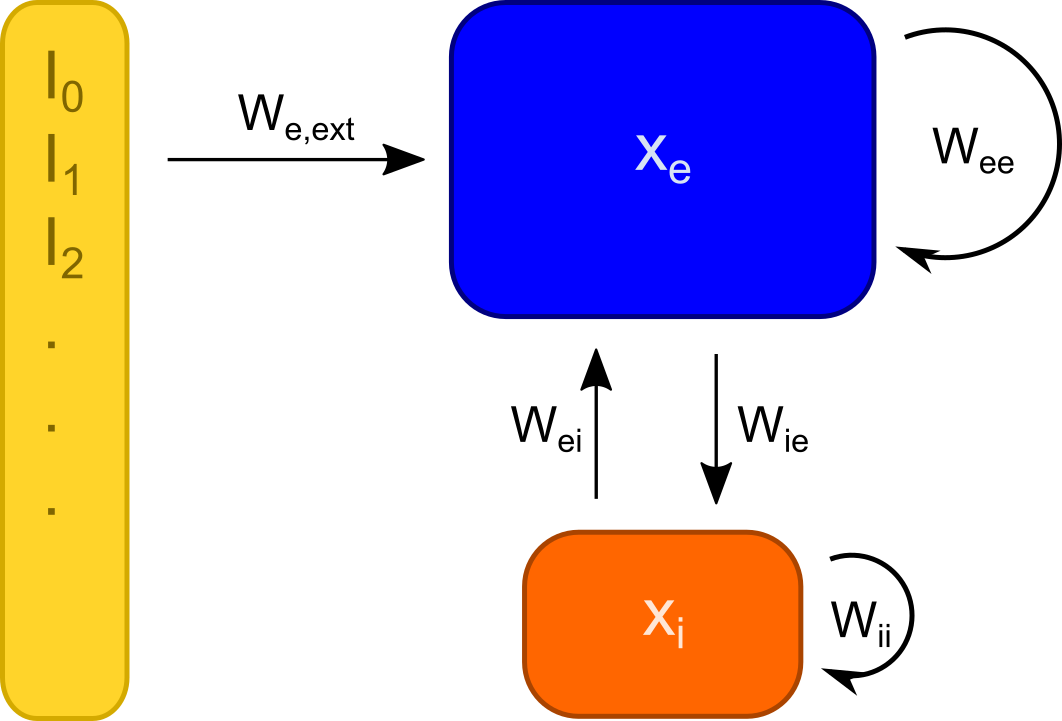
\includegraphics[width=0.7\textwidth]{../plots/illustration.png}
\caption{\label{fig:architecture} Architecture of the RNN}
\end{figure}

The recurrent network consists of a population with $N_e = 300$ excitatory units (denoted as $x_e$) and a population with $N_i = 60$ (denoted as $x_i$) inhibitory units. Furthermore, a population of $N_{ext} = 9$ excitatory units ($I_j$) is interpreted as external input, where the input coming from each external unit is to be interpreted as encoding a particular feature of a sensory stream, e.g. the recognition of a particular letter or symbol.

\section{Methods}
\subsection{Network Details}

Synaptic connectivities - represented by arrows in the illustration - were initially generated from a uniform distribution and the following properties, listed in Table \ref{tab:network_params}.

\begin{table}
\caption{Network parameters}
\begin{tabular}{l|r}
Connection Fraction $W_{ee}$ & $0.05$ \\
Connection Fraction $W_{ei}$ & $0.1$ \\
Connection Fraction $W_{ie}$ & $0.2$ \\
Connection Fraction $W_{ii}$ & $0.2$ \\
Connection Fraction $W_{e,ext}$ & $0.1$ \\
$\langle W_{e,ext} \rangle$ & $0.2$ \\
Total postsynaptic E$\rightarrow$E input & $1.0$ \\
Total postsynaptic I$\rightarrow$E input & $-1.0$ \\
Total postsynaptic E$\rightarrow$I input & $1.0$ \\
Total postsynaptic I$\rightarrow$I input & $-1.0$
\end{tabular}
\label{tab:network_params}
\end{table}


\subsection{Neuron Model}

The state of the neurons is updated in discrete time steps by the following equations:

\begin{align}
x_{e,n}(t+1) &= \theta\left( \sum_{j=0}^{N_e - 1} W_{ee,nj} x_{e,j}(t) + \sum_{k=0}^{N_i-1} W_{ei,nk} x_{i,k}(t)  + \sum_{l=0}^{N_{ext}-1} W_{e,ext,nl} I_{l}(t) - T_{e,n}(t) + \xi_{e,n}(t) \right) \\
x_{i,n}(t+1) &= \theta\left( \sum_{j=0}^{N_e - 1} W_{ie,nj} x_{e,j}(t) + \sum_{k=0}^{N_i-1} W_{ii,nk} x_{i,k}(t)  - T_{i,n}(t)  + \xi_{i,n}(t)\right)
\end{align}

where $\theta(\cdot)$ is the theta function and $T_e$ and $T_i$ represent additional threshold values. $\xi_{e/i}$ are random noise terms sampled from a Gaussian distribution at each time step with parameters $\mu_{noise,e/i}$ and $\sigma_{noise,e/i}$.

To stabilize network activity, each neuron's threshold is updated each time step such that the neuron's average activity approach a given target value:

\begin{equation}
T_{e/i,n}(t+1) = T_{e/i,n}(t) + \mu_{IP}\left(x_{e/i,n}(t)-r_{target,e/i,n}\right)
\end{equation}

where $\mu_{IP}$ is the learning rate of this ``intrinsic plasticity". Target rates $r_{target,e/i}$ were drawn randomly from a Gaussian distribution with parameters $\mu_{target,e/i}$ and $\sigma_{target,e/i}$ for each neuron and kept fixed throughout the simulation.

Parameters of the dynamics described in this section are given in Table \ref{tab:neuron_params}.
\begin{table}
\caption{Parameters of the neuron model}
\begin{tabular}{ll}
$\mu_{noise,e}$ & $0.0$ \\
$\mu_{noise,i}$ & $0.0$ \\
$\sigma_{noise,e}$ & $0.1$ \\
$\sigma_{noise,i}$ & $0.1$ \\
$\mu_{target,e}$ & $0.1$ \\
$\mu_{target,i}$ & $0.1$ \\
$\sigma_{target,e}$ & $0.0$ \\
$\sigma_{target,i}$ & $0.0$ \\
$\mu_{IP}$ & $0.002$
\end{tabular}
\label{tab:neuron_params}
\end{table}


\begin{comment}
<!--
w_mean_pre_ext_input = .2

w_exc_min = 0.0001
w_inh_max = -0.0001
##

## Neuron
g_neur = 20. # gain factor of the activation function

r_target_e_mu = 0.1 # mean homeostatic excitatory target firing rate
r_target_e_sigm = 0.#2 # standard deviation of homeostatic excitatory target firing rate
r_target_set_e = np.minimum(1.,np.maximum(0.,np.random.normal(r_target_e_mu,r_target_e_sigm,N_e)))

r_target_i_mu = 0.1 # mean homeostatic inhibitory target firing rate
r_target_i_sigm = 0.#2 # standard deviation of homeostatic inhibitory target firing rate
r_target_set_i = np.minimum(1.,np.maximum(0.,np.random.normal(r_target_i_mu,r_target_i_sigm,N_i))) 

mu_IP = 0.002 # threshold adaption rate

T_e_max_init = 1.
T_i_max_init = 1.

mu_mem_noise = 0.
sigm_mem_noise = np.sqrt(0.01)
##

## Synaptic Normalization
w_total_ee = .5#*N_e**.5 # total presynaptic E->E input
#w_total_eext = .5 # total presynaptic Ext->E input
w_total_ei = -1.#*N_i**.5 # total presynaptic I->E input
w_total_ie = 1.#*N_e**.5 # total presynaptic E->I input
w_total_ii = -1.#*N_i**.5 # total presynaptic I->I input
##
\end{comment}

\subsection{Rules of the Input Sequence}

In each time step, only a single unit is in its active state $I_j(t) = 1$. The sequence of active input nodes was generated by a markov chain with transition probabilities shown in Fig. \ref{fig:grammar_markov}.

\begin{figure}
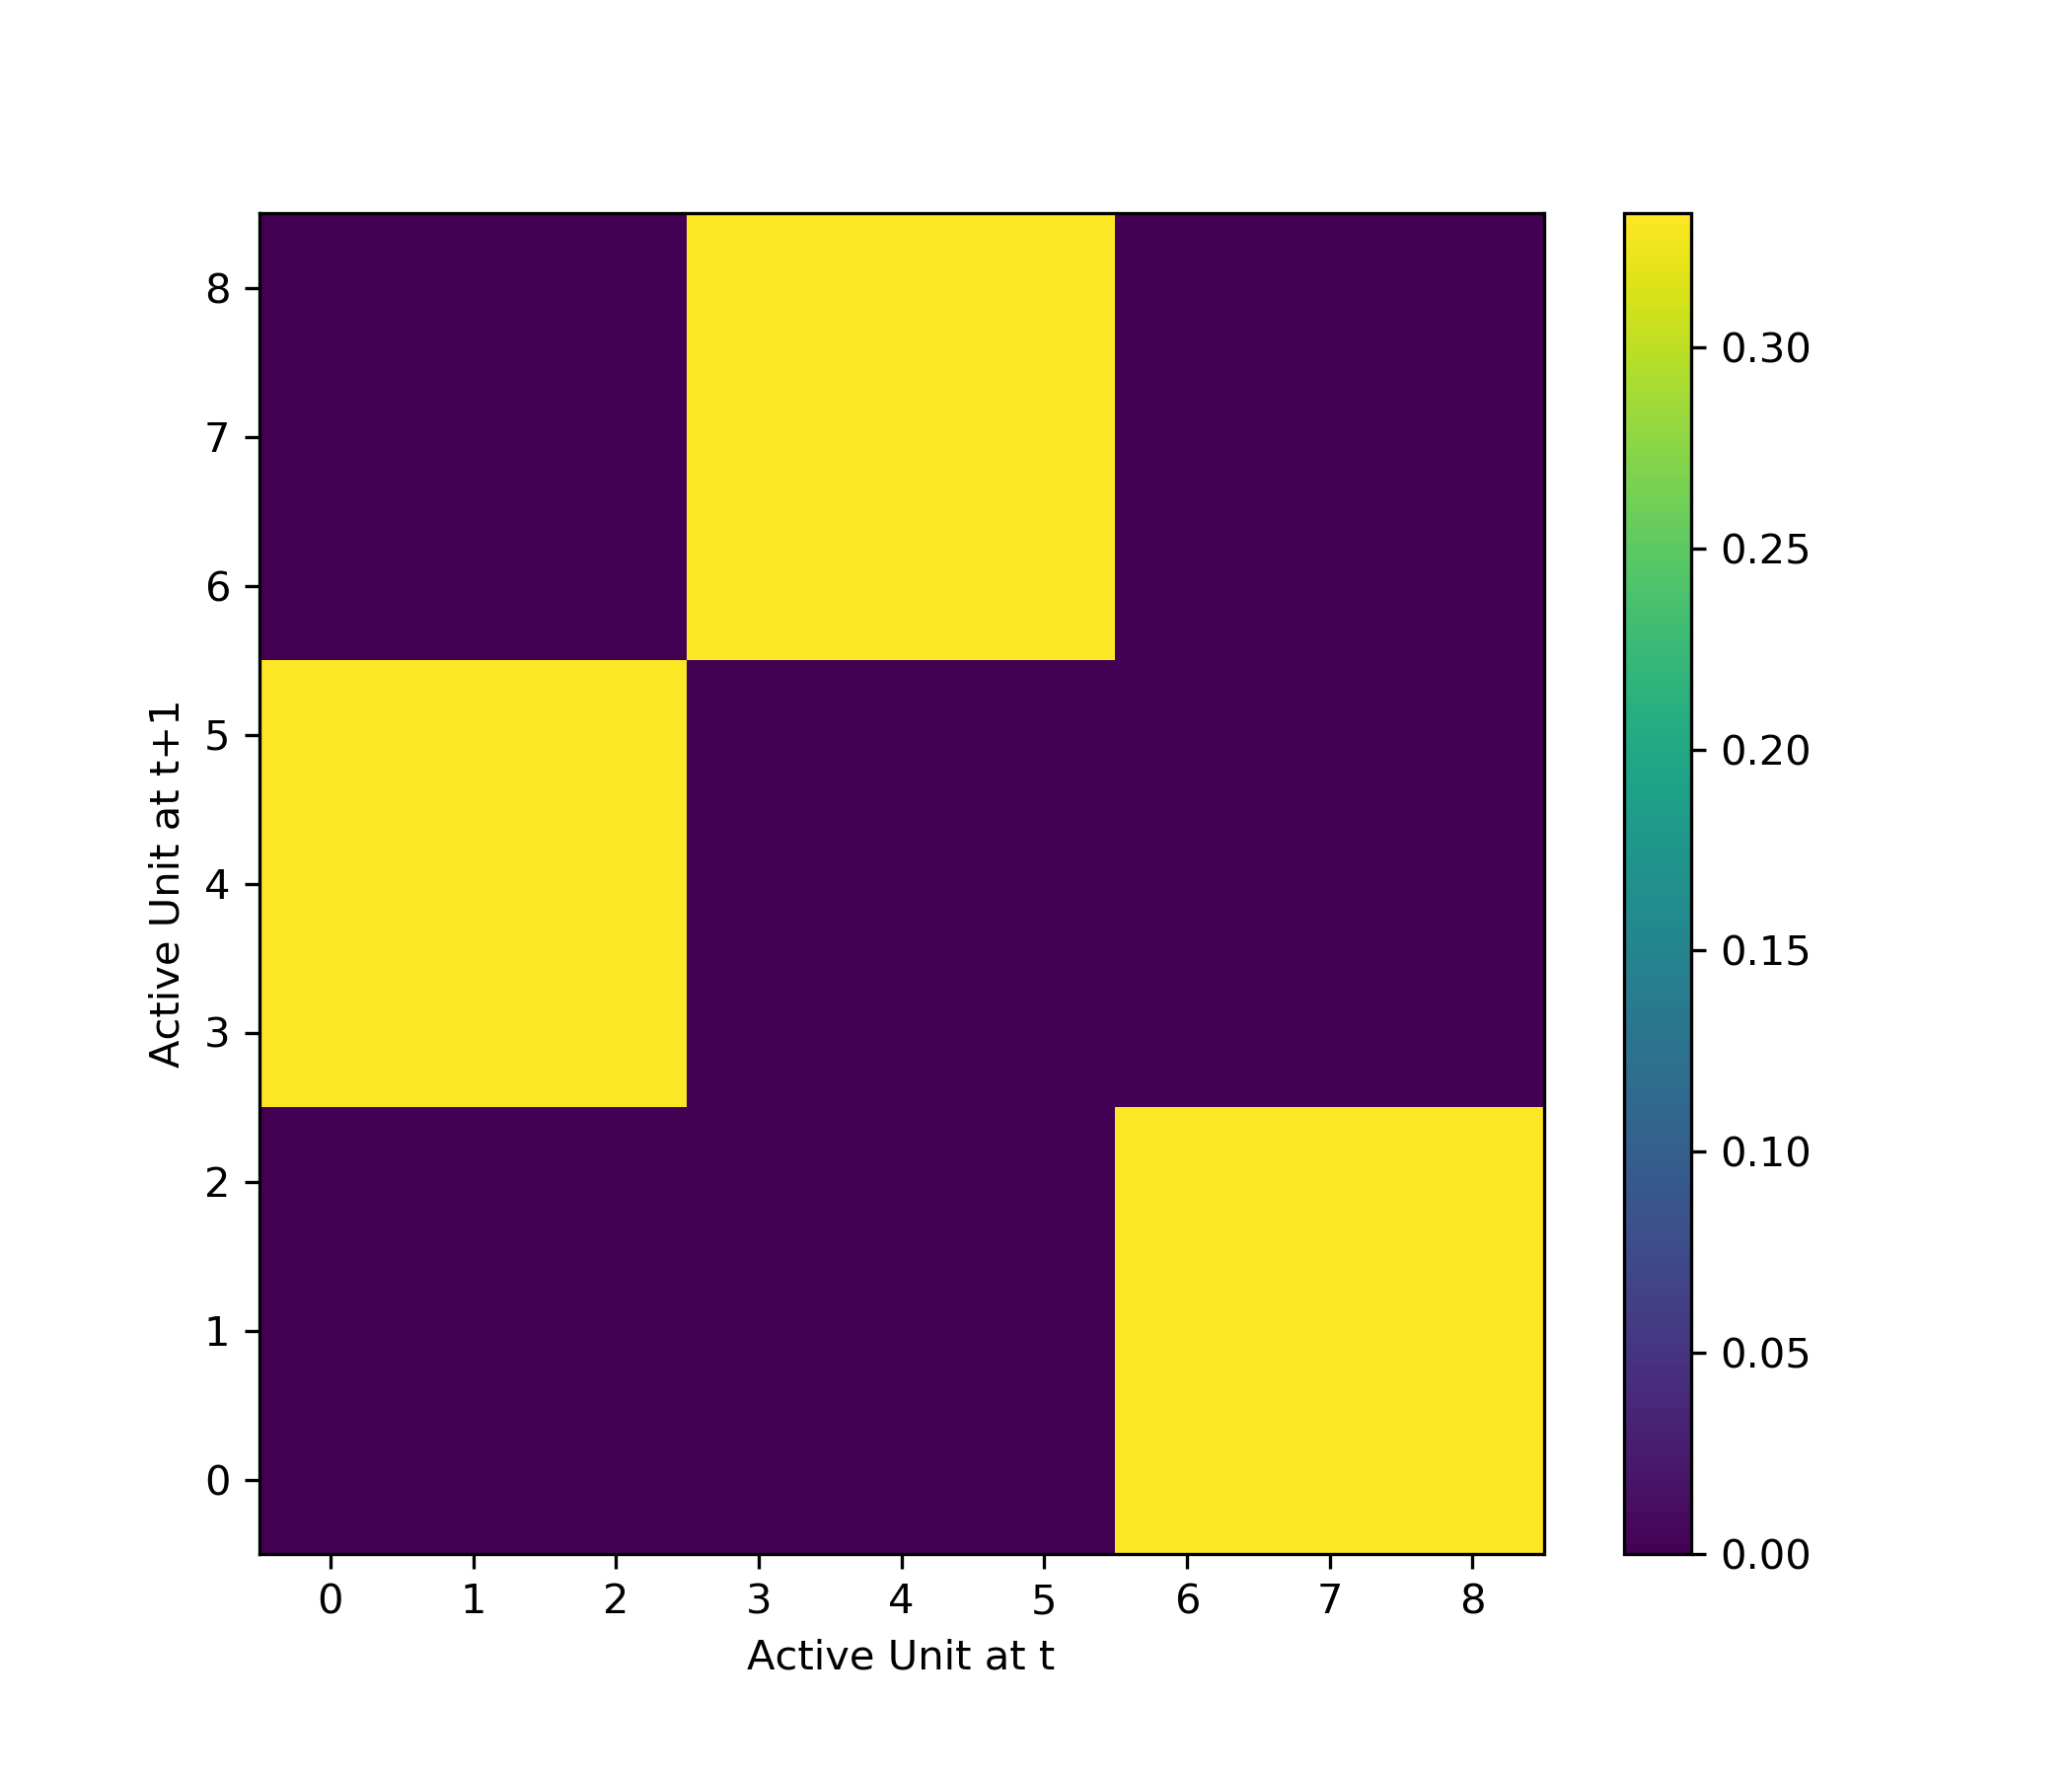
\includegraphics[width=\textwidth]{../plots/Grammar_Markov.png}
\caption{\label{fig:grammar_markov} Transition Matrix between subsequently active input states}
\end{figure}

Due to the structure of the transition matrix, the sequence is partially predictable in the sense that an element of $\{0,1,2\}$ will always be followed by an element of $\{3,4,5\}$ etc.

\subsection{Plasticity Rules}

Recurrent excitatory connection were subject to two plasticity mechanisms: A simple pre-post Hebbian learning rule and a postsynaptic multiplicative normalization preventing connectivity runaway.

\begin{align}
\Delta W_{ee,ij}(t) &= \mu_{hebb} \left( x_{e,j}(t-1)x_{e,i}(t) - x_{e,i}(t-1)x_{e,j}(t) \right) \\
W_{ee,ij}(t) &= w_{total,ee}\frac{W_{ee,ij}(t-1) + \Delta W_{ee,ij}(t)}{\sum_{k=0}^{N_e - 1} W_{ee,ik}(t-1) + \Delta W_{ee,ik}(t)}
\end{align}

We did not include pruning or creation of synapses, but set a very small lower bound for existing excitatory connections.

\section{Results}

Network activity settled at a constant mean rate and a corresponding mean treshold, see Fig. \ref{fig:pop_act_time} and Fig. \ref{fig:thresholds_time}. 

\begin{figure}
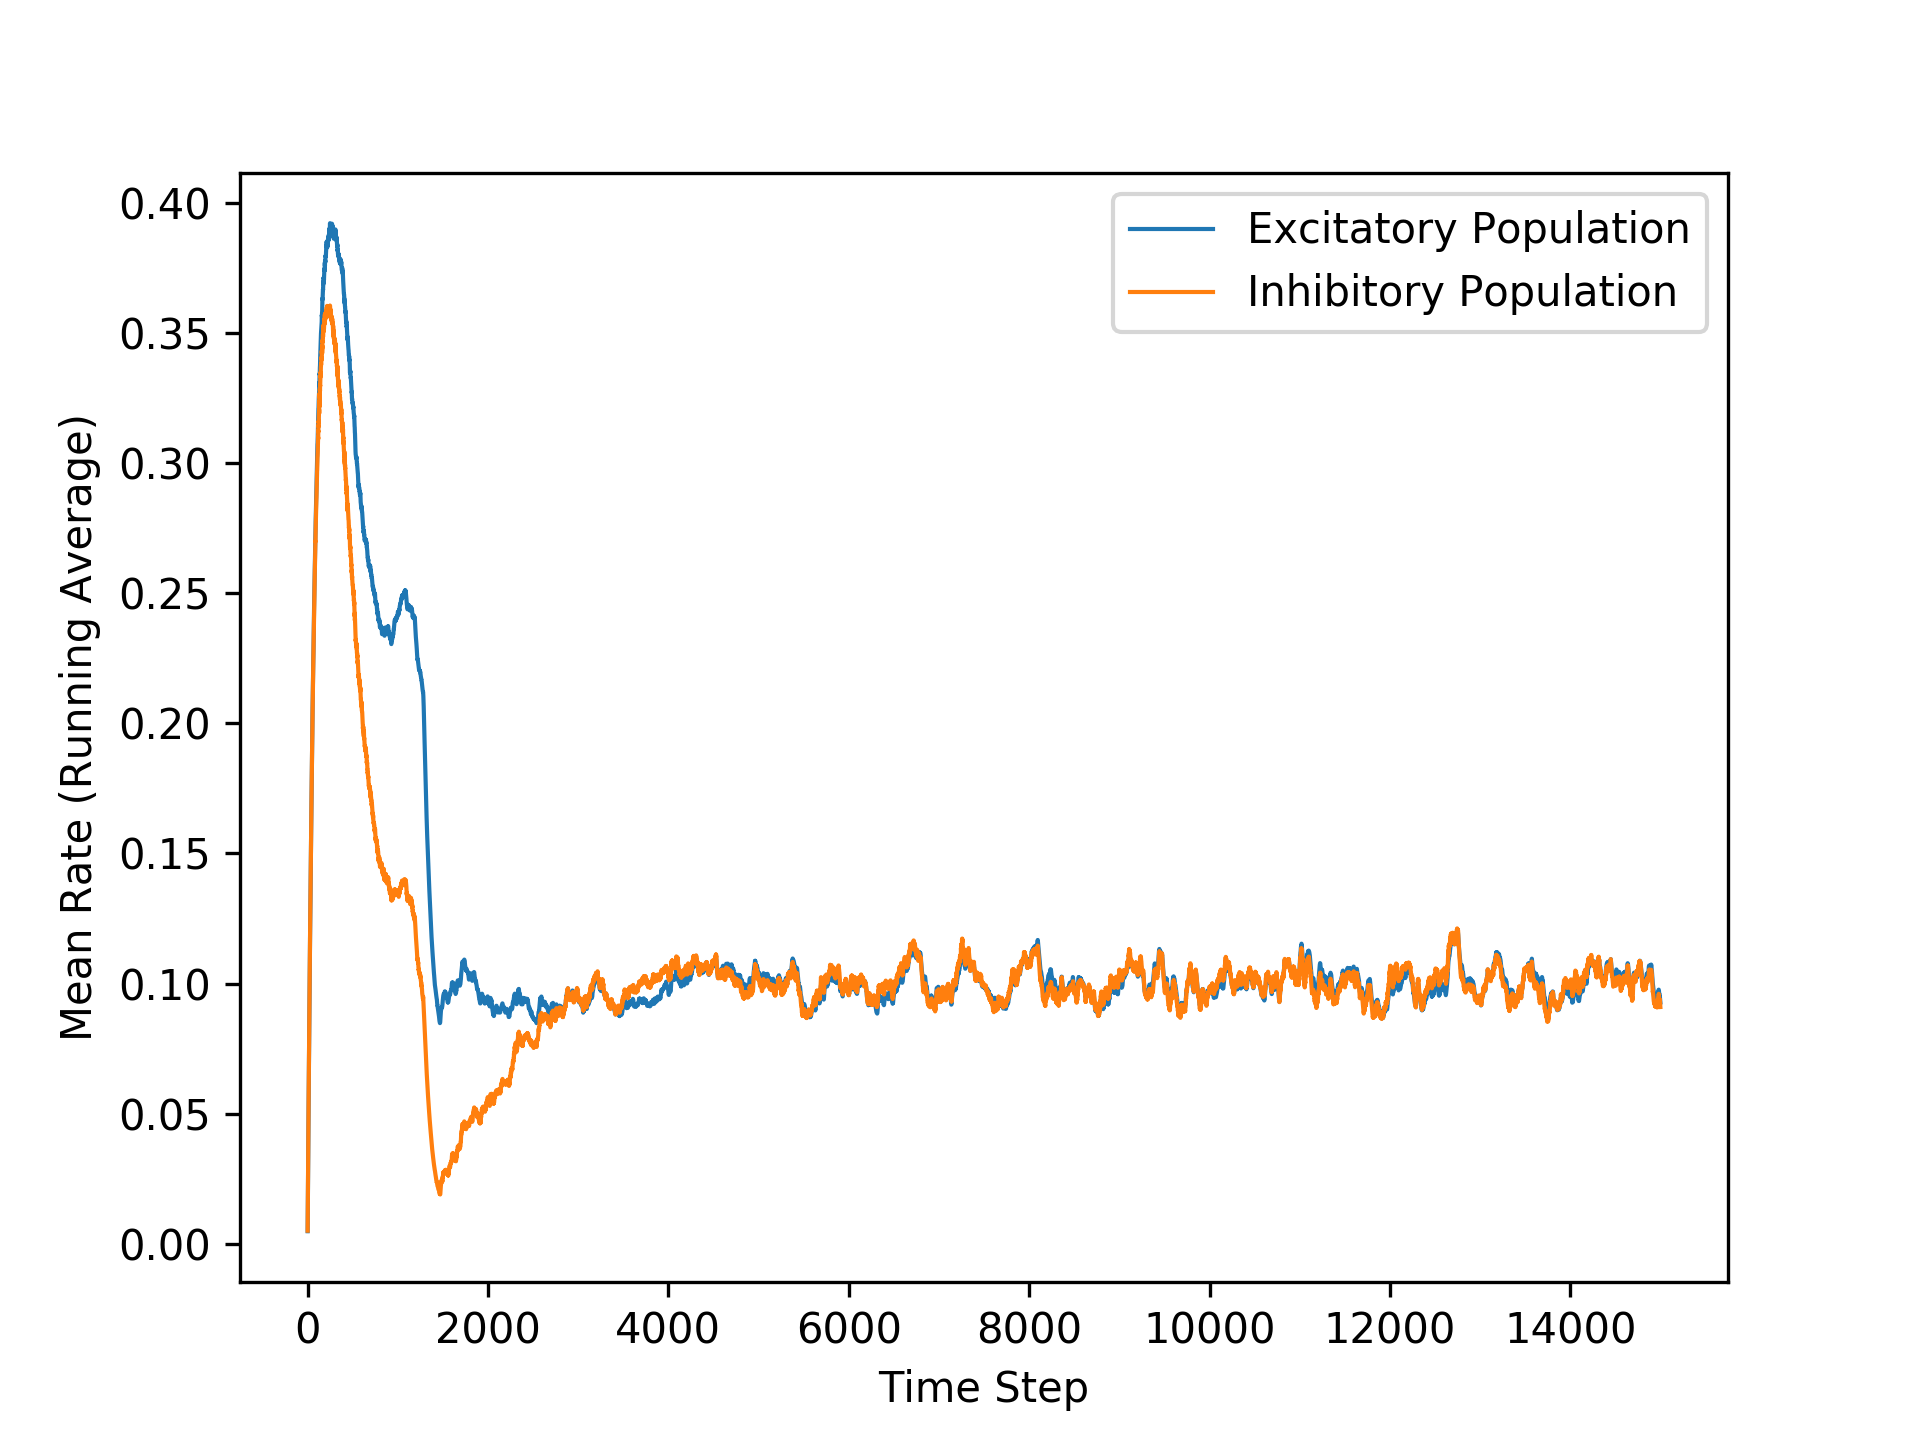
\includegraphics[width=\textwidth]{../plots/pop_act_time.png}
\caption{\label{fig:pop_act_time} Running average of excitatory and inhibitory population activity.}
\end{figure}

\begin{figure}
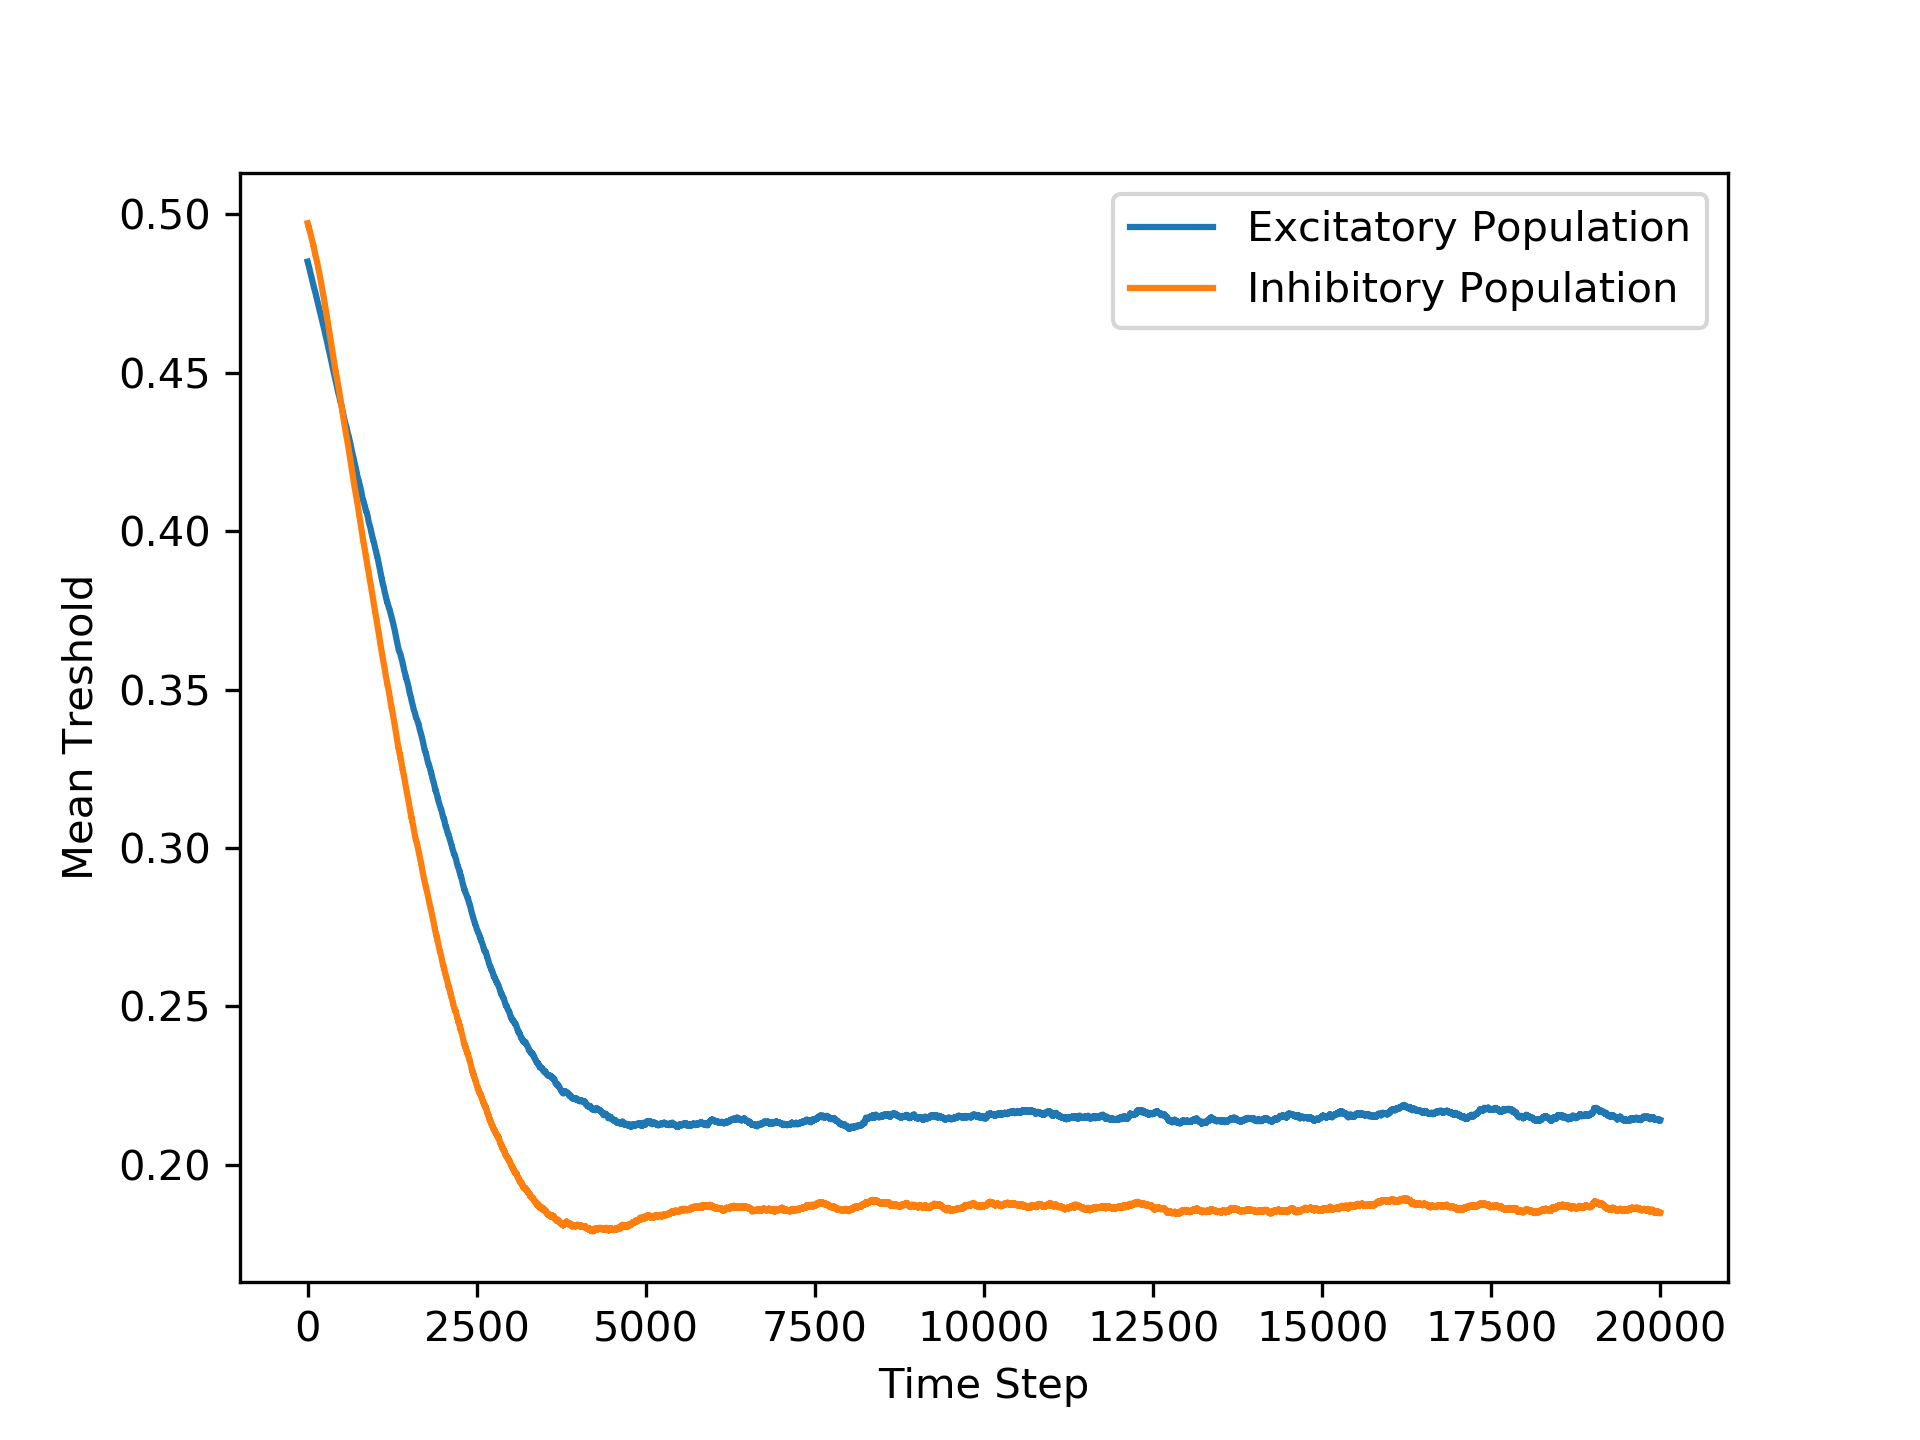
\includegraphics[width=\textwidth]{../plots/thresholds_time.png}
\caption{\label{fig:thresholds_time} Population mean of excitatory and inhibitory thresholds.}
\end{figure}

Furthermore, Fig. \ref{fig:act_raster} and Fig. \ref{fig:isi_dist} suggest that the appearance of active states follows poissonian statistics. However, the distribution of excitatory inter``spike"-intervals shows a clear preference for multiples of 3, which was not present in the absence of external input and is reflected in the 3-fold periodicity of the input sequence. 

\begin{figure}
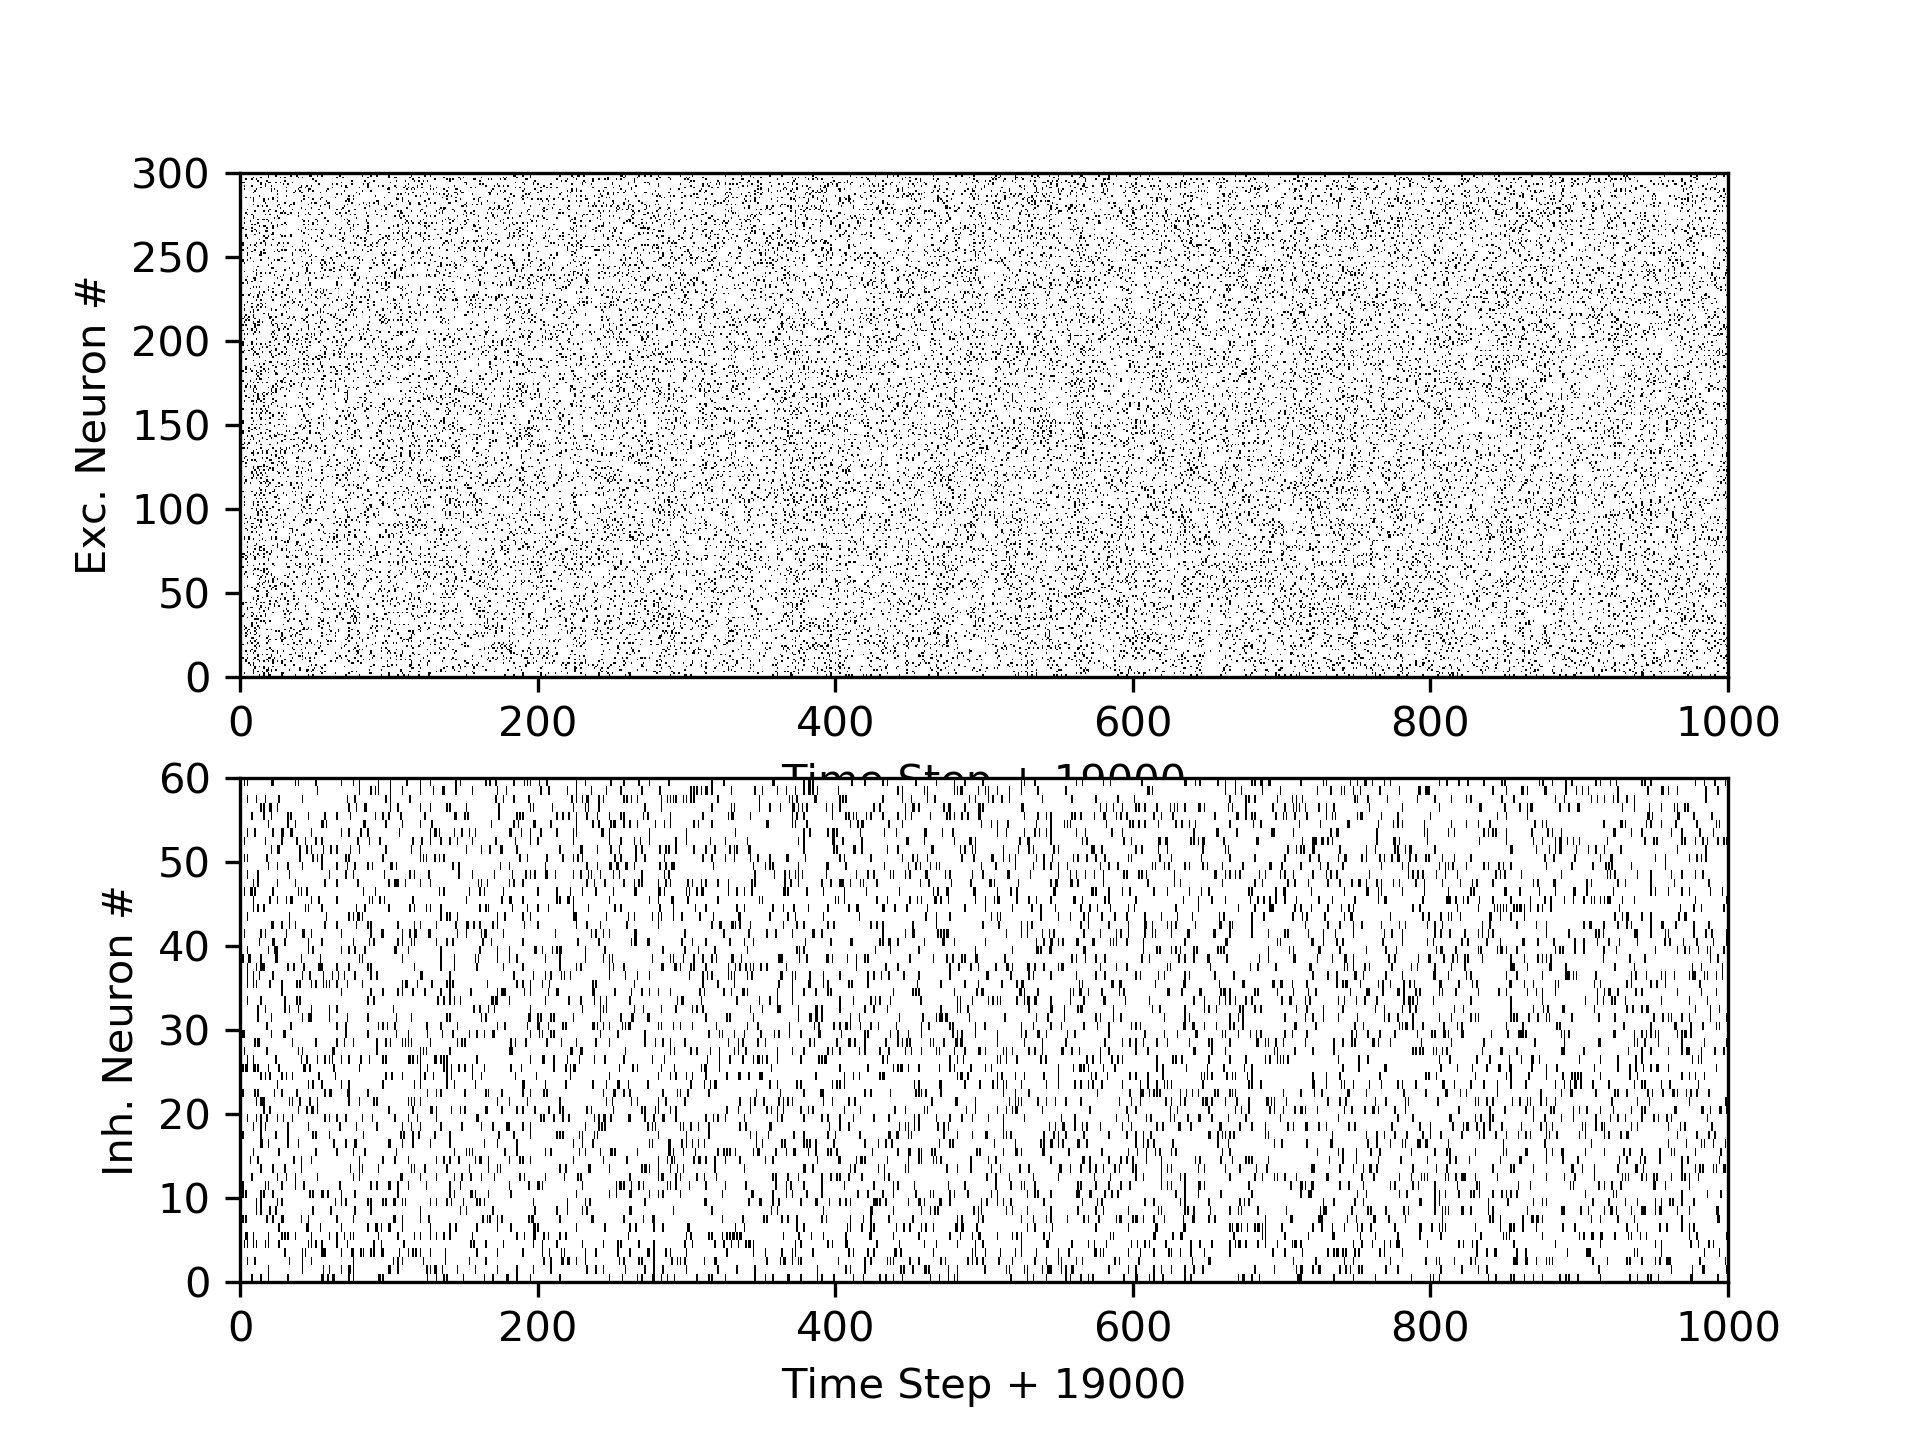
\includegraphics[width=\textwidth]{../plots/act_raster.png}
\caption{\label{fig:act_raster} Raster plot of network activity.}
\end{figure}

\begin{figure}
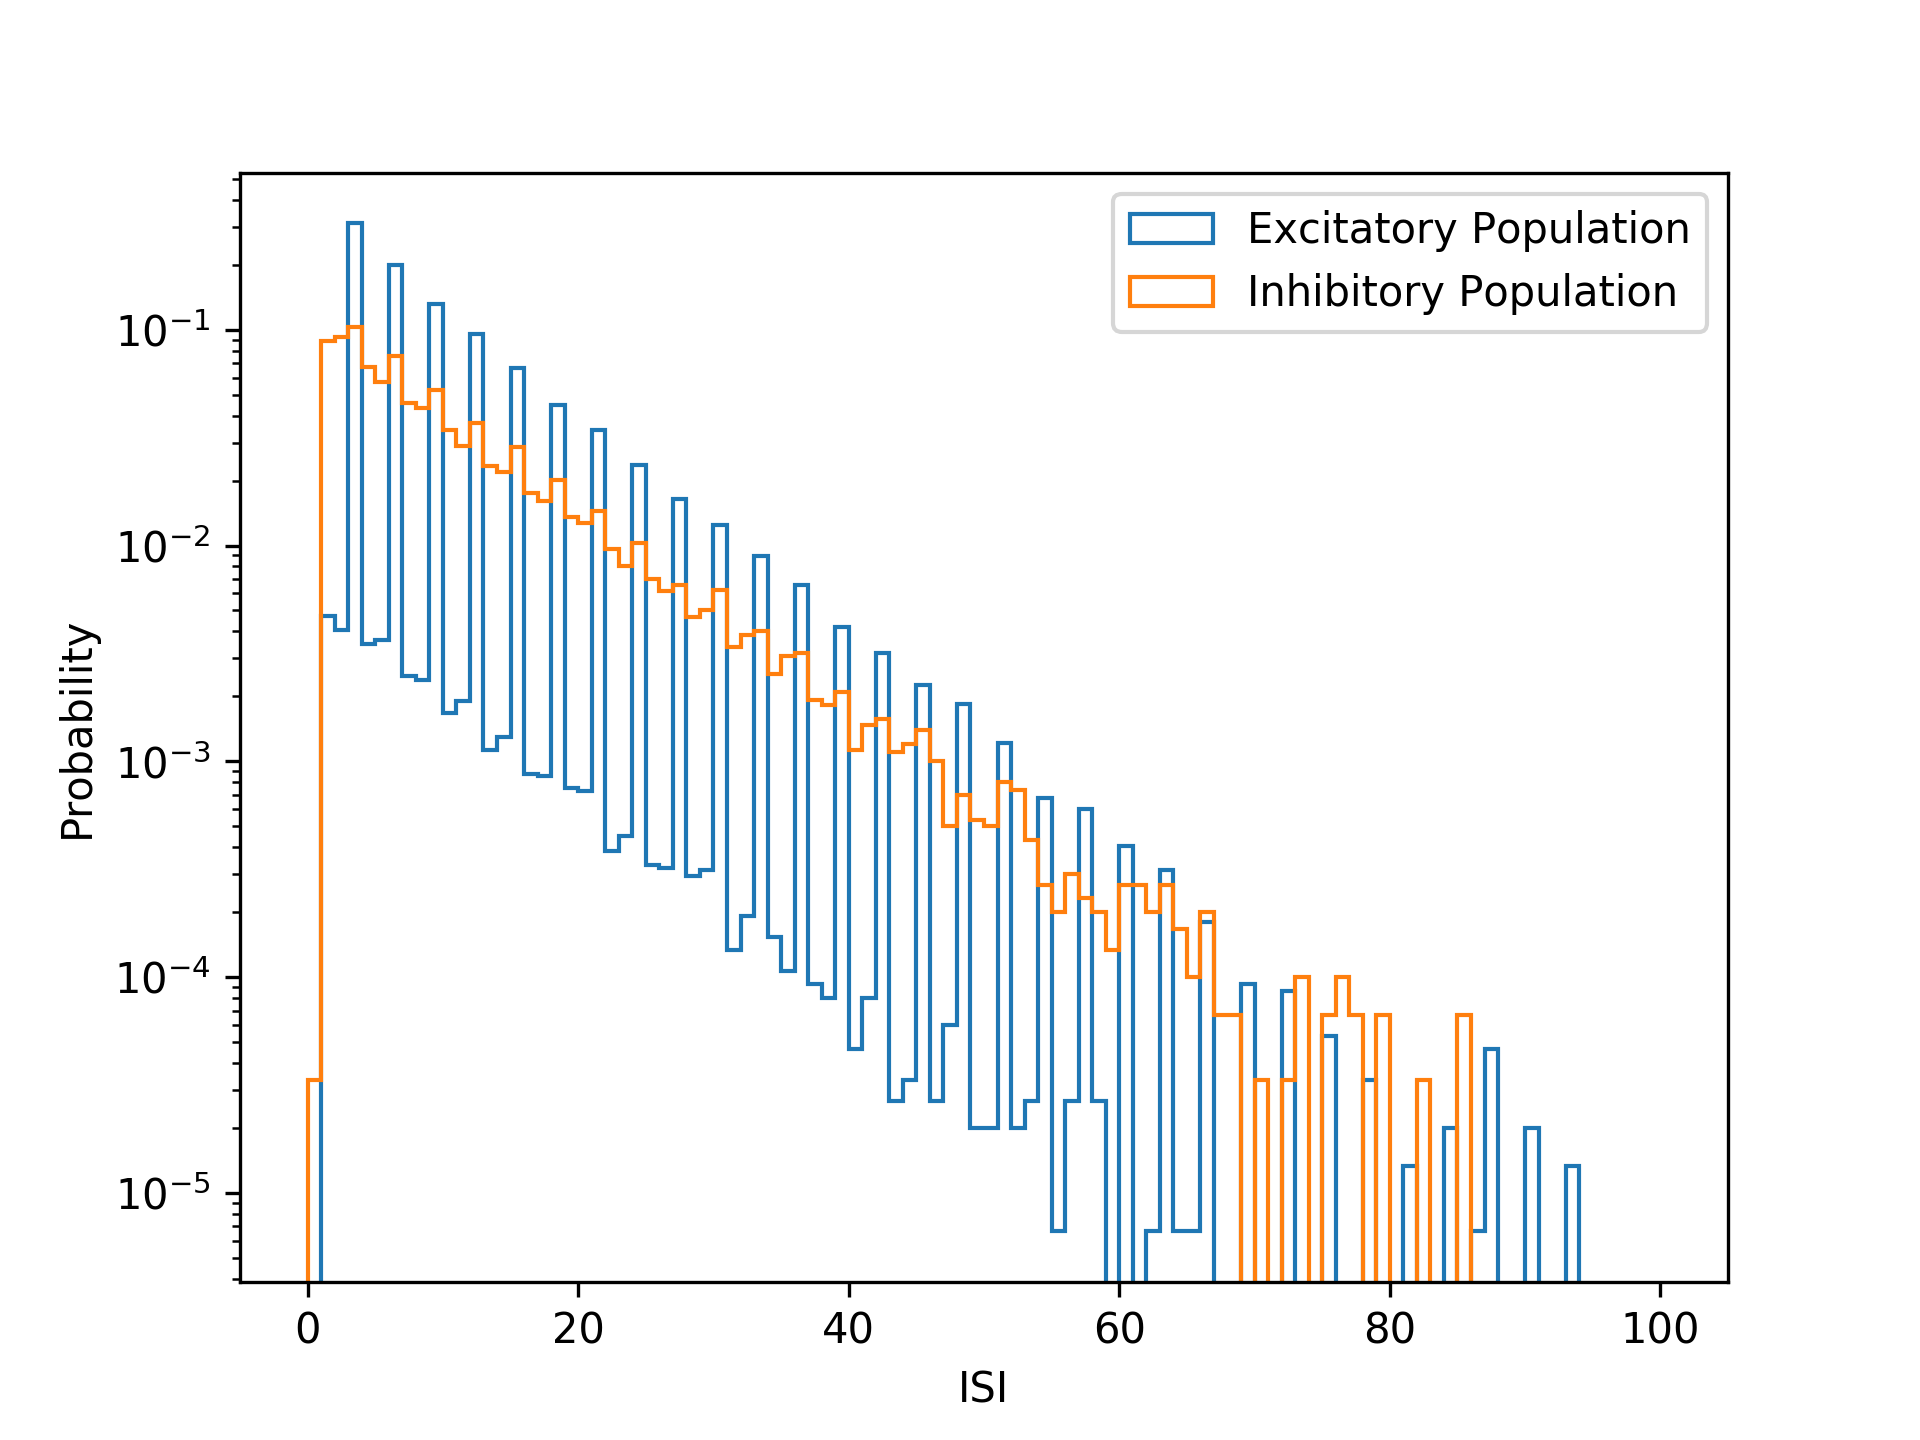
\includegraphics[width=\textwidth]{../plots/isi_dist.png}
\caption{\label{fig:isi_dist} Distribution of interspike intervals.}
\end{figure}

Generally speaking, the implemented plasticity rules often gave rise to time courses of synaptic weights similar to the one shown in Fig. \ref{fig:w_ee_sample_time}: the emergence of one or more comparably strong weights alongside a majority of weak connections.

\begin{figure}
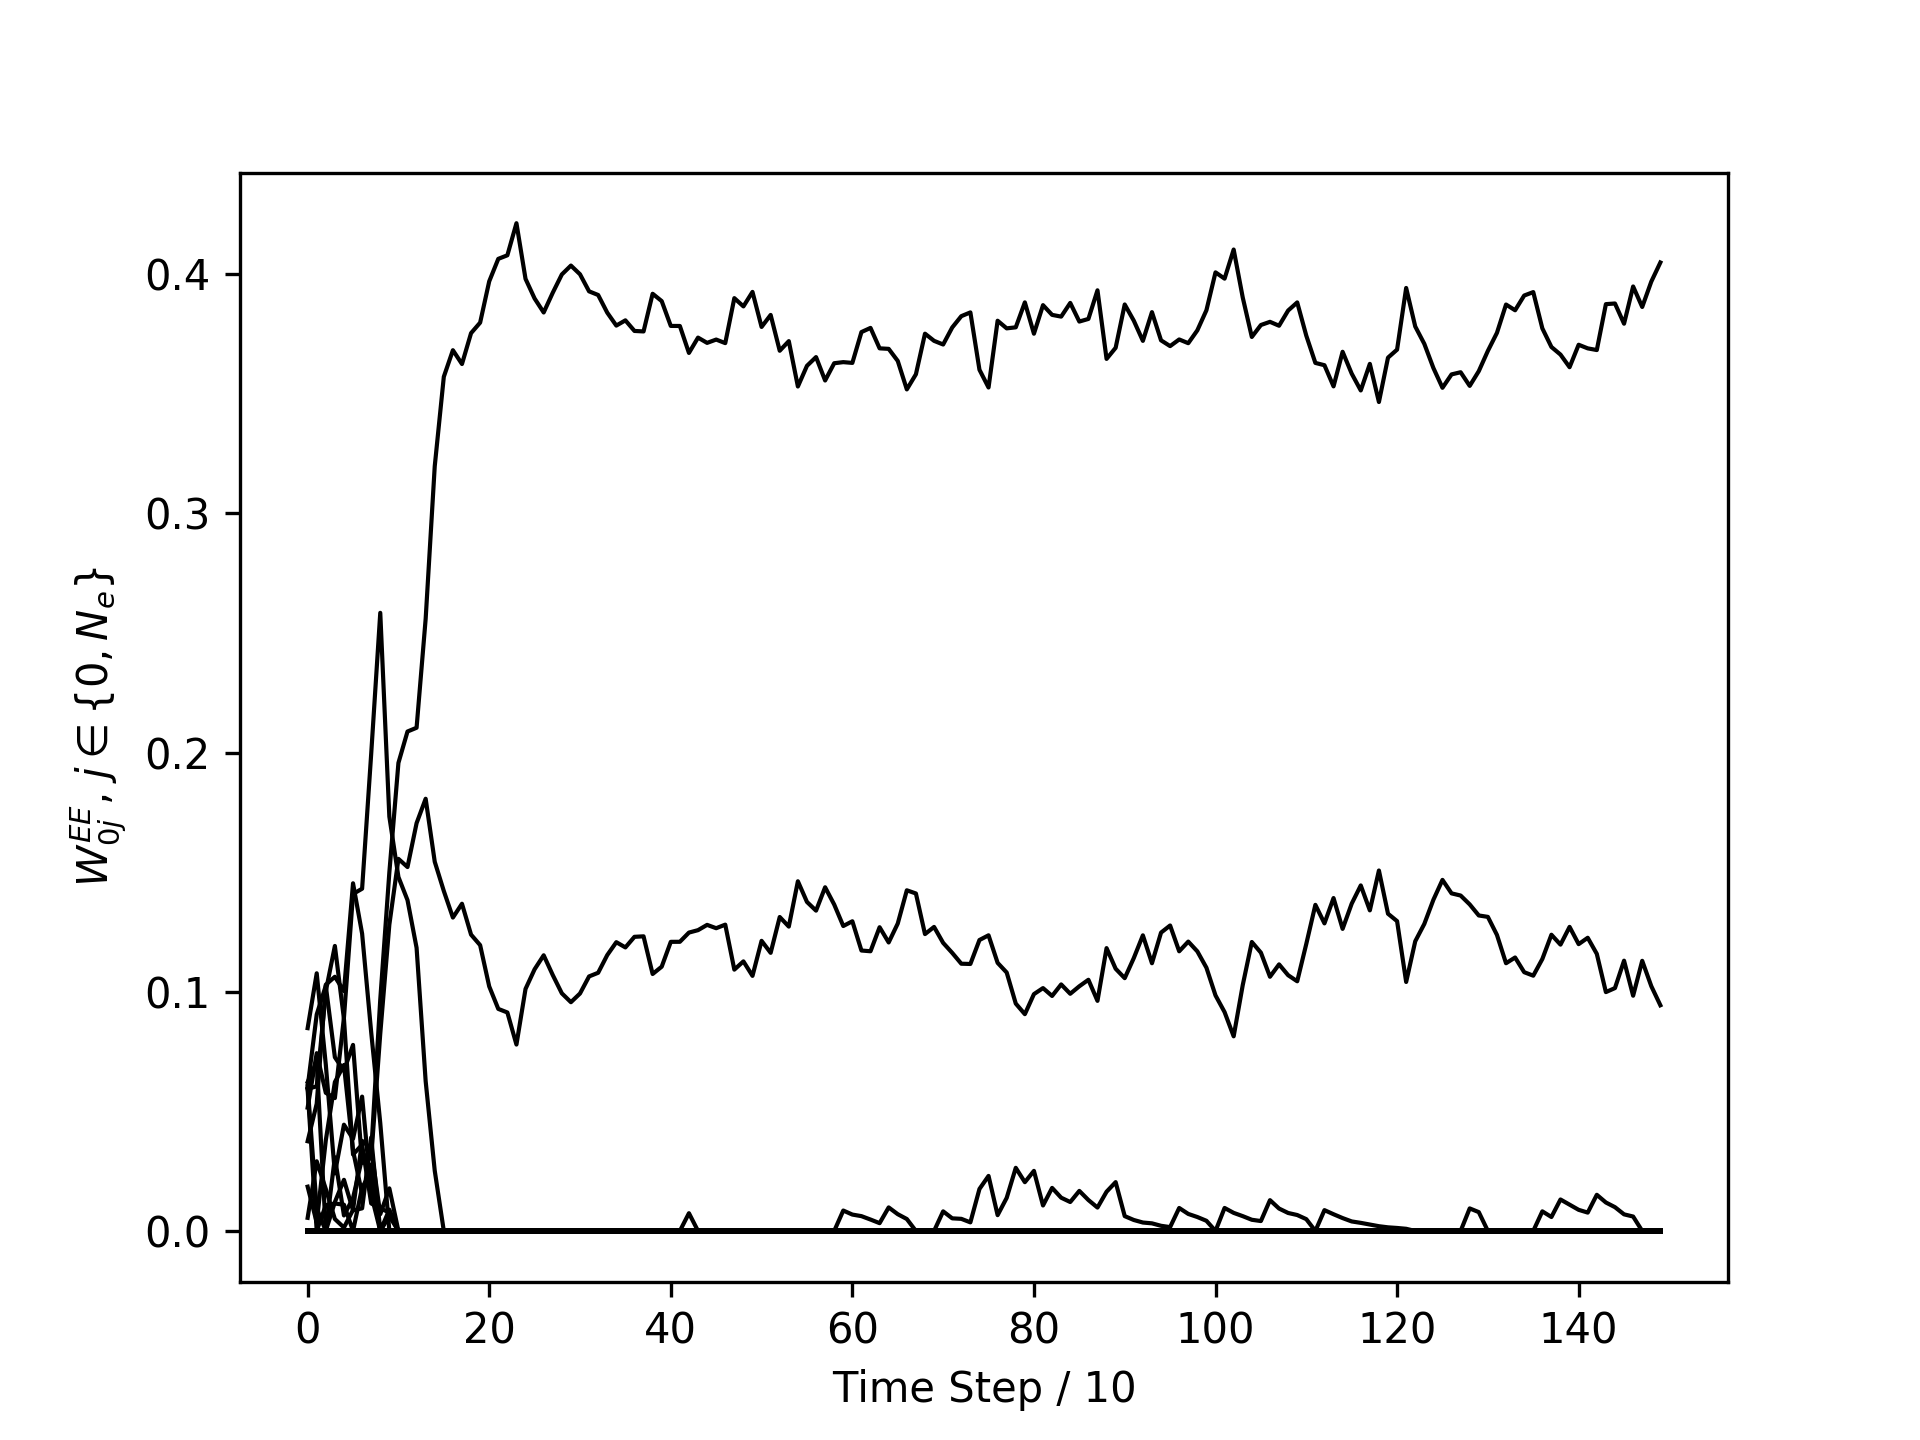
\includegraphics[width=\textwidth]{../plots/w_ee_sample_time.png}
\caption{\label{fig:w_ee_sample_time} Sample time course of E->E weights.}
\end{figure}

\subsection{Cluster Analysis of Excitatory Activity}

Following the conceptual idea presented by Elman \cite{Elman_1990}, we performed a hierarchical cluster analysis of the binary activity vectors of the exitatory population. For this, we used the activity data of $x_e$ from the last $t range analysis[1]-t range analysis[0]$  steps. We then performed a hierachical cluster analysis with Ward's method. The resulting dendrogram is depicted in Fig. \ref{fig:act_dendrogram}. A 3-fold structure is visible in the uppermost branching layer.

\begin{figure}
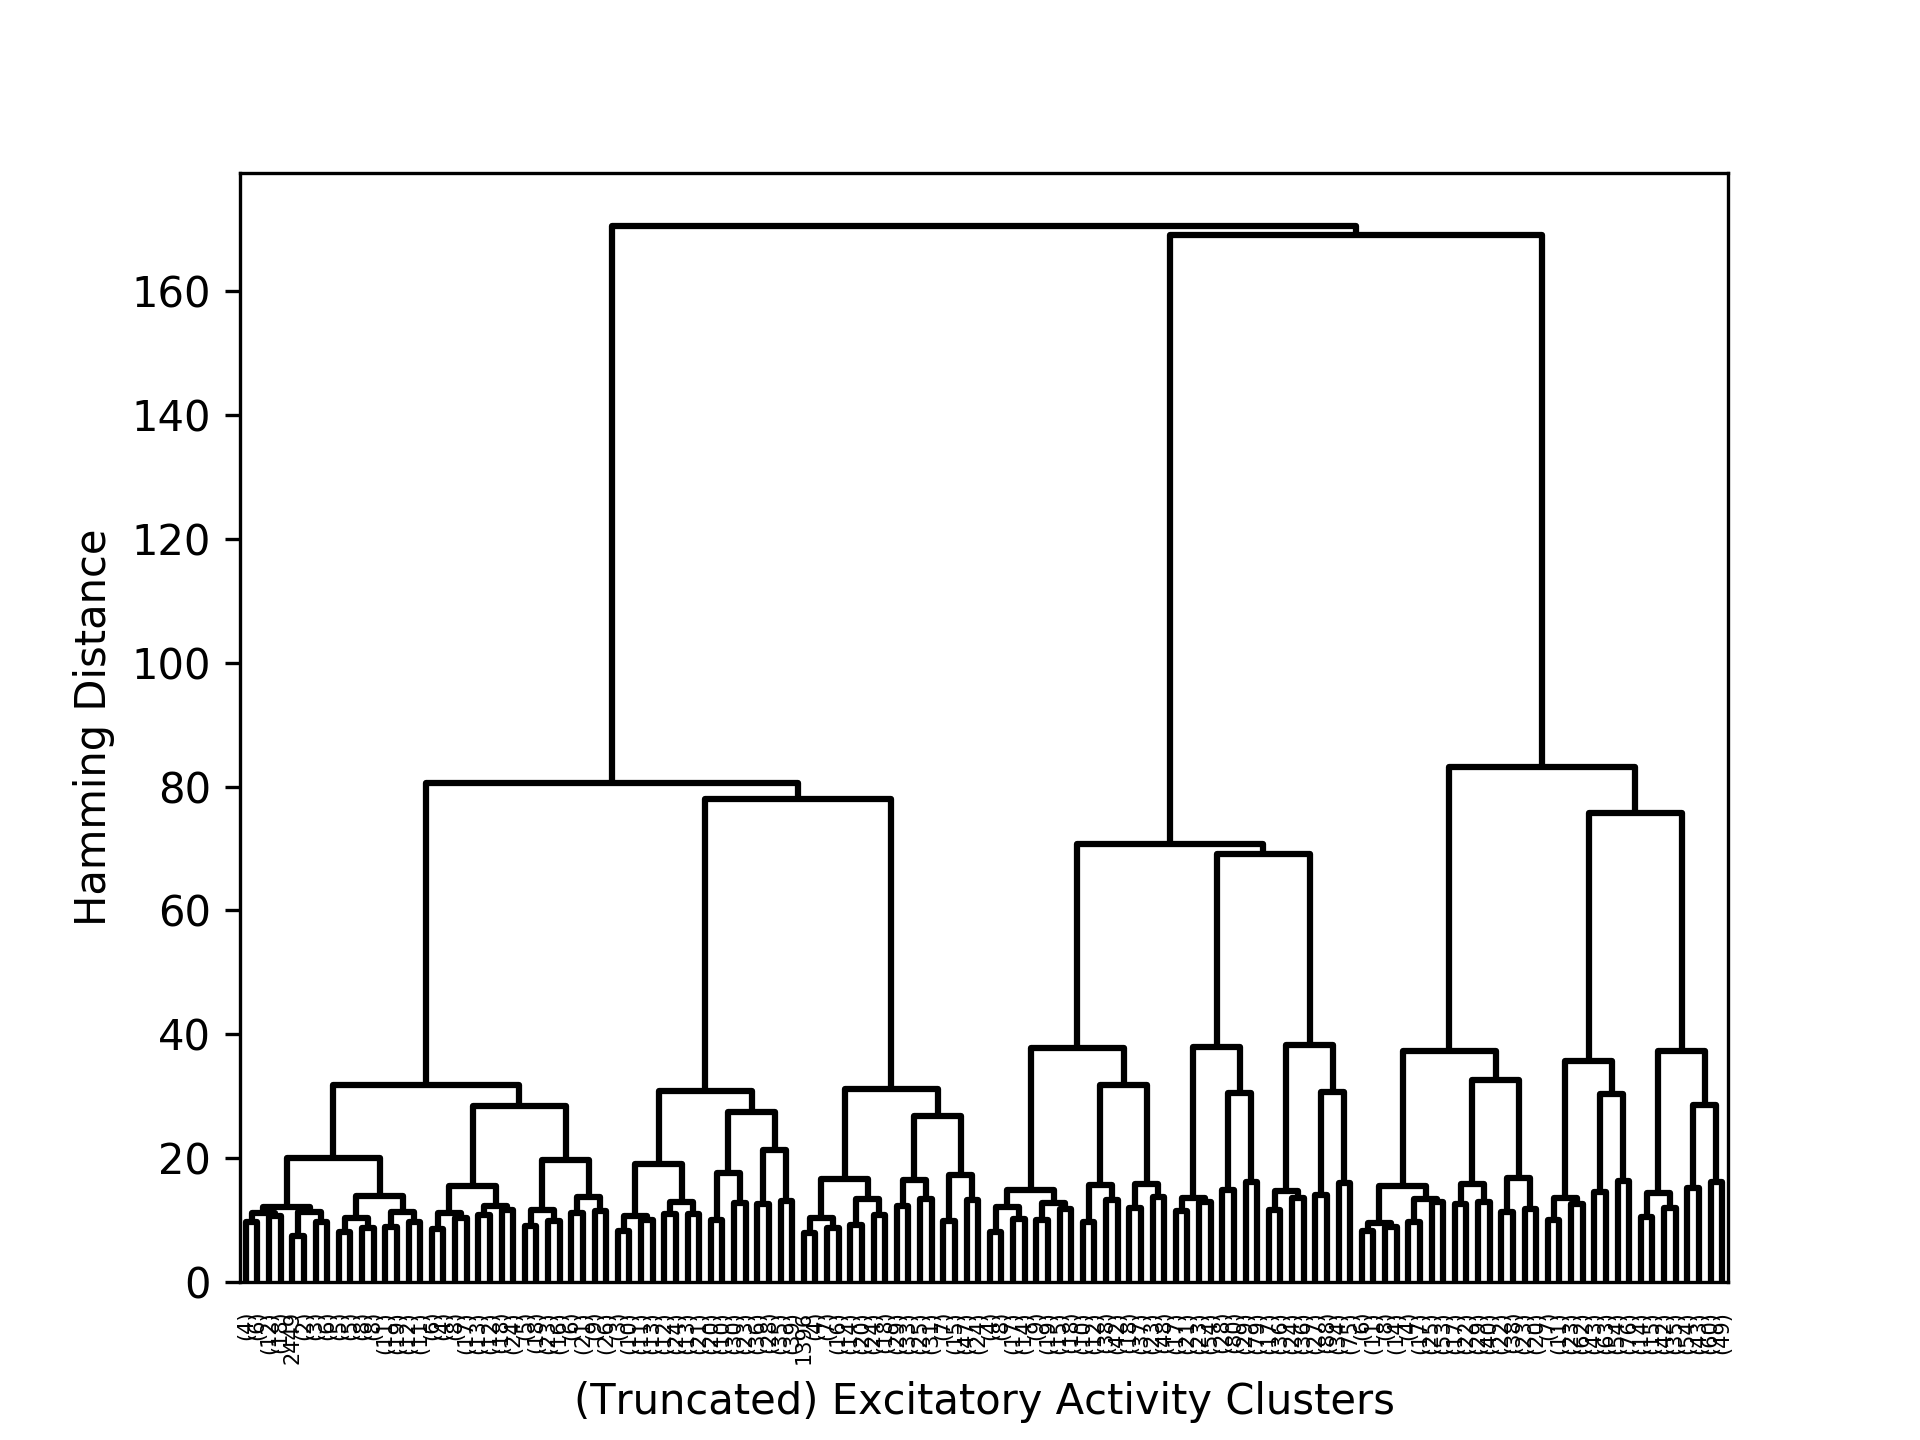
\includegraphics[width=\textwidth]{../plots/act_dendrogram.png}
\caption{\label{fig:act_dendrogram} Dendrogram of a cluster analysis of excitatory activity patterns.}
\end{figure}

\bibliographystyle{unsrt}
\bibliography{../code/ipynb_biblio}

\end{document}